\section{Introduction}
\section{Tools}
\subsection{IDE}
Visual Studio Code was used for this project due to prior experience with the IDE. It is also one of the most popular tools in the industry 
as shown by the Stack Overflow Developer Survey\cite{StackOverflowDeveloper} and the TOP IDE Index\cite{TOPIDETop}.
VS Code has excellent support for many programming languages, and with a wealth of community made extensions there are many tools to aid with development.
\subsection{Version Control}
Version control is a system that records changes to a file or set of files over time so that you can recall specific versions later.\cite{GitVersionControl}
Using version control with an external hosting provider also makes working over several computers easy which will be useful for this project, and it ensures everything is backed up remotely.
Git was chosen for version control as it is the industry standard, with GitHub being used as the hosting provider.
\subsection{Database Visualisation}
Neo4j has two tools for database visualisation as part of the AuraDB web interface; Bloom and Browser. Bloom is used to 
visualise the data in a graph as has been discussed in the design chapter previously. Browser is used to test CYPHER queries on the database.
CYPHER is the query language created by Neo4j for retrieving data from their graph databases. As shown in the screenshot below, the user can enter a 
query and have the data returned as a graph, table (represented as a series of JSON objects), raw text and as code (JSON objects).
This is useful for quickly testing CYPHER queries and debugging database interactions.
\begin{figure}[h]
    \centering
    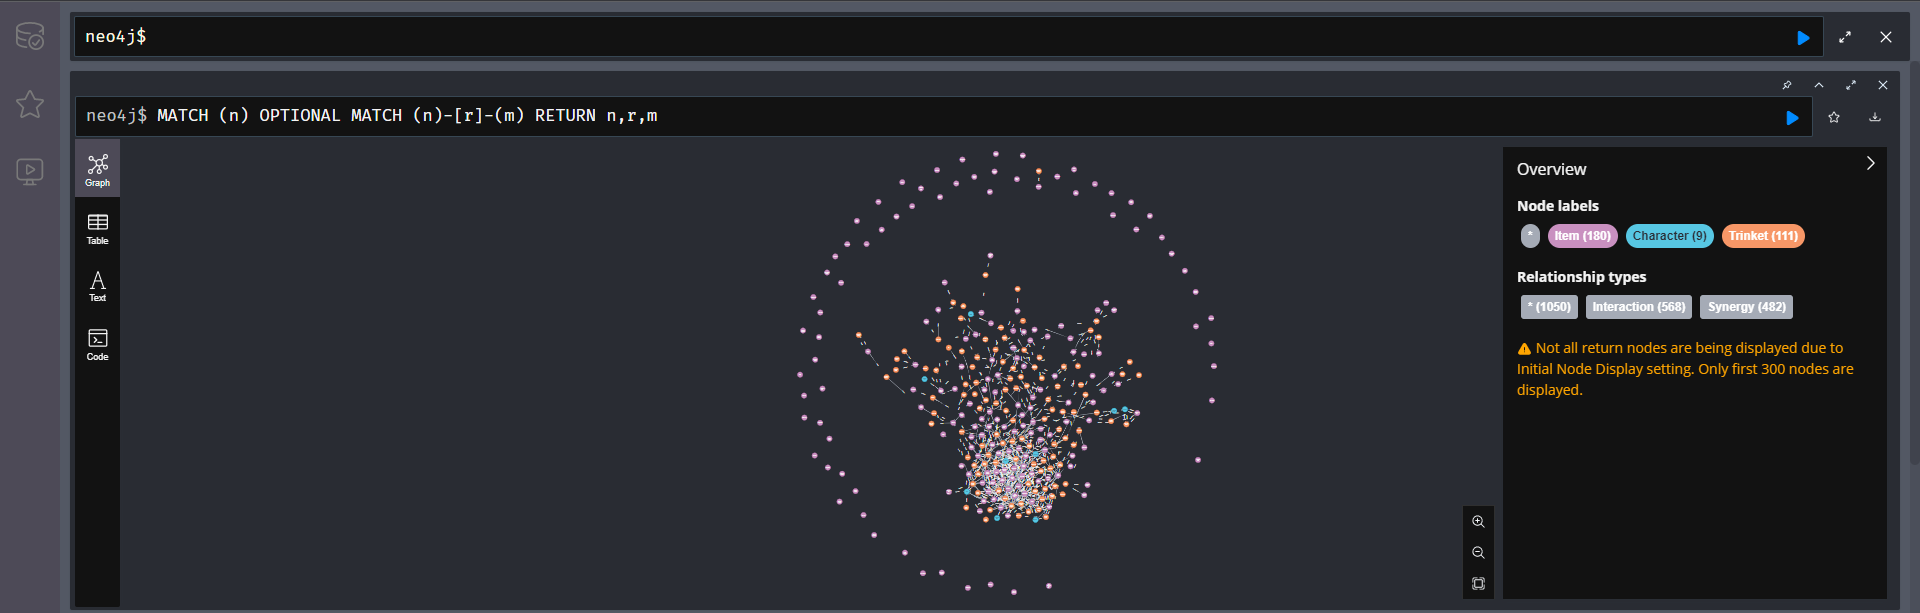
\includegraphics[width=0.8\textwidth]{neo4jBrowser}
    \caption{AuraDB Browser}
\end{figure}
\subsection{Libraries}
\subsection{Client Side}
\begin{description}
    \item[Cytoscape] A JavaScript library that `allows you to easily display and manipulate rich, interactive graphs'\cite{franzCytoscapeJsGraph2016}. 
    Used in this project to display the data in graphs to the user.
    \item[Material] An Angular specific library containing material design componenets, used in this project to quickly create UI componenets.
\end{description}
\subsection{Server Side}
\begin{description}
    \item[Neomodel] used to create models for getting data from neo4j database
    \item[django-cors-headers] allows in browser requests to djano application from other origins
    \item[djangorestframework] 
\end{description}
\section{Data Processing}
this section covers getting the data needed to create the database and creating the database
\subsection{Finding Data Source}
fandom wikis all should have an xml dump available on the special:statistics page
It isnt always up to date, so i had to request a update
while waiting for that I looked at other BOI sources such as platinum god and the game files

got the xml file and its massive and not consistently formatted
it's set up like a huge list of pages but theres not order to them and sometimes random stuff is added in between them
looked challenging to extract data from so looked towards other games i.e. pokemon
however that wiki didn't have a dump at all and i got no response regarding getting one
other data sources for pokemon exist but each have their own issues
\subsection{Data Extraction}
while looking for alternative sources and waiting on response from wiki admins worked on extracting the data
used beautifulsoup to parse the xml tags and traverse the data
Used the items collection page to get the names of all the items locate the correct xml elements
trinkets and characters(?) had to be hardcoded as a complete list didnt exist in the xml

beautifulsoup is used to traverse the data and get the 'text' child of all the relevant 'pages'
then regex is used to grab the relevant sections from the text
\subsection{Cleaning the Data}
regex is used again to clean the sections of text
The text contains lots of tags for vairous features in the wiki such as dlc tags and links to other pages
turns bullet pointed lists into nested arrays
\subsection{Importing into Database}
neo4j has a data importer tool which uses csv files to populate a data model
csv files were generated from the data objects in python
\begin{figure}[H]
    \centering
    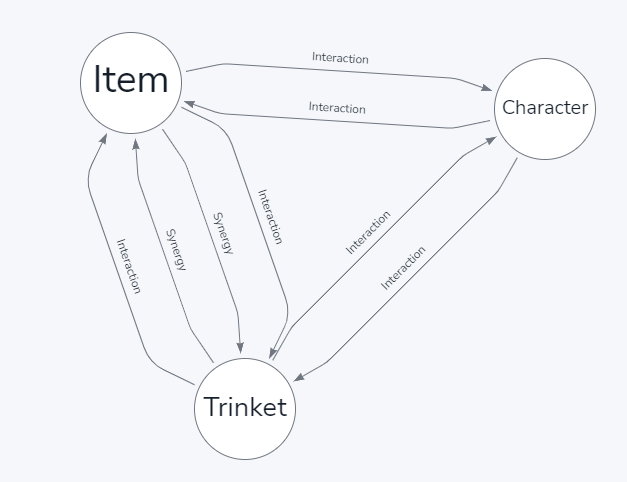
\includegraphics[scale=0.4]{dataImport}
    \caption{Database Model in Neo4j Data Importer}
\end{figure}
\section{Web Stack}
creating django project with an api app and a main "query" app
api app contains webserver (?) and the settings
each app then contains the the models, views and urls etc
urls.py defines what functions get called by each urls
views.py defines the functions used by urls, these functions contain all the functionality the user interacts with,
each function takes in a request from the url and depending on the type of request (e.g get, post etc), performs the relevant action
models.py contains classes each of which represent a type if data entity

create a angular project and any components
(explain angular project structure)
each component represents a "screen"
(explain component structure)

There is a shared services file, this defines the interaction with the backend api
the address of the backend server is defined in there and the functions that make the http requests

each project has it's own git repo which are then submoduled into the main project repo
\section{Database Interaction}
Used neomodel to define classes for each entity and relationship type, these classes contain methods for retrieving data
Getting all nodes is very easy due to built in methods, however these do not exist for relationships
so to get all relationships you have to perform a cypher query to get them
\section{Client Side}
first made tables to check everything worked
found that the json like object created by neomodel couldn't be interpreted by the front, so had to manually make a get method for each class
This causes getting large amounts of data (relationships) to take quite a long time

I created a second component to show the data in a graph form as per my initial design
To do this I used cytoscape.js (more info)
had to rewrite how the data is formatted when sent to the front end so that it matchs what cytoscape expects
still takes a long time to get data from backend 
so decided to write it to a json file so at least for quicker debugging it can load directly from the file
tweaked some settings to make the graph easier to read

\section{Conclusion}